\documentclass[12pt]{report}

\usepackage{graphicx}
\graphicspath{ {figures/} }
\graphicspath{{images/}}
\usepackage[margin=1 in, includefoot]{Geometry}
\usepackage{hyperref}
\hypersetup{colorlinks=true,linkcolor=blue,urlcolor=cyan,}
%pdfpagemode=fullScreen}
\usepackage[english]{babel}
\usepackage[utf8]{inputenc}
\usepackage{fancyhdr}
\pagestyle{fancy}
\fancyhf{}
\renewcommand{\headrulewidth}{0pt}
\renewcommand{\footrulewidth}{1pt}
\usepackage{ragged2e}
\usepackage{times}
\usepackage{array}
\renewcommand\thesection{\arabic{section}}
\usepackage {hyperref}
\usepackage{graphicx,wrapfig,lipsum}
\usepackage{array}
\usepackage{multirow}

%header and footer
\cfoot{\fontsize{10}{12} \selectfont DYPIT, Department of Computer Engineering 2022-2023 }
%\chead{Cloud Cryptography: User End Encryption}




\begin{document}

%Start of Title page

\centering \large \textbf  {A PRELIMENERY REPORT ON   }\\
\vspace{0.9 cm}
\Large \textbf{"PC Game Development using Unity”}\\
\vspace{0.5 cm}
%\normalsize {on}\\
%\vspace{0.1 cm}
\normalsize{SUBMITTED TO THE SAVITRIBAI PHULE PUNE UNIVERSITY, PUNE}\\
\normalsize{IN THE PARTIAL FULFILLMENT OF THE REQUIREMENTS}\\
\normalsize{  FOR THE AWARD OF THE DEGREE}\\
\vspace{0.8 cm}
\normalsize {Of}\\
\vspace{0.8 cm}

\Large\textbf{BACHELOR OF COMPUTER ENGINEERING}\\
\vspace{0.9 cm}
\large{SUBMITTED BY}\\
\vspace{0.3 cm}

\large \textbf  {Ankur Patil (BCOB10)}

\large \textbf  {Lalu Nair (BCOB05) }

\large \textbf{Viren Patil (BCOB14)}

\large \textbf{Sharan Thakur (BCOB09)}
%\vspace{0.3 cm}


\begin{figure}[h]
\centering

\includegraphics[scale=0.25]{Logo.png }
\end{figure}

\centering \Large \textbf  {DEPARTMENT OF COMPUTER ENGINEERING}\\
\vspace{0.4cm}

\large \textbf  {DR. D. Y. PATIL INSTITUTE OF TECHNOLOGY}\\
\normalsize {PIMPRI, PUNE 411018}\\
\vspace{0.2 cm}
\large \textbf{SAVITRIBAI PHULE PUNE UNIVERSITY}\\


\large \textbf  {2022-2023}\\
\vspace{0.5 cm}

\clearpage
% End of Title page

% start of Certificate

%\begin{wrapfigure}{l}{5.5cm}
\begin{figure}[h]
\centering

\includegraphics[width=6cm]{Logo.png}
%\end{wrapfigure} 
\end{figure}

\vspace{0.3 cm}
\centering{\large \textbf{CERTIFICATE}\\}

\vspace{0.4 cm}

\normalsize{This is to certify that the Project Entitled}\\
\vspace{0.3cm}
\large\textbf{PC Game Development using Unity}\\
\vspace{0.3 cm}
\normalsize{Submitted by}\\
\vspace{0.3 cm}

\normalsize  {Ankur Patil (BCOB10)}

\normalsize  {Lalu Nair (BCOB05)}

\normalsize  {Viren Patil (BCOB14)}

\normalsize  {Sharan Thakur (BCOB09)}

\vspace{0.2 cm}
\justifying
\setlength{\parindent}{4em}
\setlength{\parskip}{1em}
\renewcommand{\baselinestretch}{1.5}
\normalsize
are bonafide students of Dr. D. Y. Patil Institute of Technology and the work has been carried 
out by them under the supervision of Mr. Sharad Adsure (Asst. Professor) and Mrs. 
Deepika Jaiswal (Asst. Professor), it is approved for the partial fulfillment of the 
requirement of Savitribai Phule Pune University, for the award of the degree of Bachelor of Computer
Engineering.

\vspace{0.4 cm}
\setlength{\parindent}{0 em}
 \textbf{Mr. Sharad Adsure}  \hspace{6.9cm}          \textbf{ Dr.Vinod Kimbahune  }   \hspace{5.5cm}         
\centering
(Internal Guide)    \hspace{6.9 cm}  ( Head of the Department)  \hspace{1 cm}    \\

\vspace{0.7 cm}
\setlength{\parindent}{0 em}
\textbf{  External Examiner}   \hspace{7cm}      \textbf    {Mrs.Sunita Patil }   \hspace{5.5cm}         
\centering
.   \hspace{10cm}  ( Project Coordinator)  \hspace{2 cm}    \\
\vspace{0.4cm}
\centering
\textbf{Dr. Lalit Kumar Wadhwa}\\
 Principal,\\
 Dr. D. Y. Patil Institute of Technology,\\
 Pimpri, Pune – 411018
\vspace{0.1 cm}
\begin{flushleft}

Date:
\end{flushleft}


\clearpage


% End of Cerficate


% start of ACKNOWLWDGEMENT

\vspace{4 cm}
\centering{\LARGE \textbf \underline{ACKNOWLEDGEMENT}\\}
\vspace{1 cm}
\justifying
\vspace{1 cm}
\justifying
\setlength{\parindent}{4em}
\setlength{\parskip}{1em}
\renewcommand{\baselinestretch}{1.5}
\normalsize
It gives us great pleasure in presenting the preliminary project report on “PC GAME DEVELOPMENT USING UNITY”


We would like to take this opportunity to thank my internal guides Asst. Prof. Sharad Adsure as well as Ms. Deepika Jaiswal for giving me all the help and guidance we needed. We are really grateful to them for their kind support. Their valuable suggestions were very helpful. 


We are also grateful to Dr. Lalit Kumar Wadhwa, Principal as well as Dr. Vinod V. Kimbahune, Head of Computer Engineering Department, Dr. D.Y Patil Institute Of Technology, Pimpri for his indispensable support, suggestions.


\begin{flushright}

\normalsize  {Ankur Patil (BCOB10)}

\normalsize  {Lalu Nair (BCOB05)}

\normalsize  {Viren Patil (BCOB14)}

\normalsize  {Sharan Thakur (BCOB09)}
\end{flushright}
\clearpage
%end of Acknoledgement
 
% start of ABSTRACT
\vspace{4 cm}
\centering{\LARGE \textbf \underline {ABSTRACT}}\\
\vspace{1 cm}
\justifying
\setlength{\parindent}{4em}
\setlength{\parskip}{1em}
\renewcommand{\baselinestretch}{1.5}
\normalsize
The 2D (Dodgeball Video Game) is a multiplayer game written in Unity 3D using C\#. The game allows players to play over a network, locally with friends on the same network, or over the internet via Photon Cloud. The game plays as you would expect from a dodgeball game. Players can run around, pick up balls, and throw them at each other. If the player is hit enough times, the player is eliminated. Players can choose to continue the game or stop at the end of the game. This game is made with assets and different packages that users can enjoy! This "dodgeball video game" aims to appeal to a market that is still under-tapped. There are already several examples of dodgeball games on the market, but none are perfect and each has some compromises. Some with great interaction with the field, but leave room for variables such as ball/player skill, etc. Proper implementation will keep our users intrigued  and provide a great and unique gaming experience Our main desire is to analyze the existing small market and build on previous dodgeball game attempts to develop a never-before-seen and unique dodgeball experience. Being able to reproduce the game and take advantage of the technology here today will help produce new life into the game dodgeball. Although it will not be 100 percent similar to the original game we all played as kids, the same basic principle of working together as a team to eliminate the enemy team is still present.

\raggedright{ \textbf \underline{KEYWORDS : }}Unity 2D, Game Development, Mono Behaviour, C\#, Real–World, Object Oriented Programming, WEBGL, iOS

\clearpage
% end of  ABSTRACt


% Start of table of content

\tableofcontents
\clearpage
% end of table of content

% Start of table of figures
\listoffigures
\thispagestyle{empty}

\clearpage
\pagenumbering{arabic}

\fancyhead[R]{\thepage}
% end of table of figures

% INTROUDCTION
\centering
\section{INTRODUCTION}
\raggedright
\subsection{OVERVIEW}

\justifying
\setlength{\parindent}{4em}
\setlength{\parskip}{0.5em}
\renewcommand{\baselinestretch}{1.5}

\normalsize
\hspace{1.7cm}
This engineering project report details the development of "The Infinite Pleasure", a multiplayer dodgeball video game created using Unity and the Photon Unity extension. The game offers an immersive and interactive experience for players, allowing them to choose their character, map, and compete with friends on the same local network.

The game follows traditional dodgeball rules, with players picking up balls, running around, and throwing them at each other. The game employs a server-client relationship to handle essential concepts such as rendering, player data, and network connectivity.

"The Infinite Pleasure" offers a unique twist to the classic dodgeball game, with innovative gameplay mechanics that would be impossible to replicate in real life. Players are placed into teams, and their objective is to catch, dodge, and launch the ball into the air to eliminate the opposing team.

The game's matchmaking system ensures that players with similar or slightly higher experience levels are paired together. This report outlines the development process, including the game's mechanics design, network architecture, and matchmaking system.

Overall, "DogeBall" combines the fun and chaotic gameplay of dodgeball .With its multiplayer features and Unity integration, it offers an enjoyable and competitive gaming experience for players to engage in virtual doge-themed dodgeball matches.




\clearpage

\raggedright
\subsection{ Motivation}

\justifying
\setlength{\parindent}{4em}
\setlength{\parskip}{0.5em}
\renewcommand{\baselinestretch}{1.5}
\normalsize\hspace{1.7cm}\begin{itemize} \item We are living at the cusp of modern technology with pocket computers with us (our smartphones), in our leisure time, all of us reach into our smartphones to play the next big game to pass time.

\item Being the students we are and wanting to play the latest and greatest games; which drives us to build a unique mechanic for the multiplayer systems.

\item A game is much more than just its software. It has to provide a much more enjoyable experience.

\item Not enough good dodgeball games free-to-play.\\
\end{itemize}
\raggedright
\subsection{Problem Definition}

\justifying
\setlength{\parindent}{4em}
\setlength{\parskip}{0.5em}
\renewcommand{\baselinestretch}{1.5}
\normalsize \hspace{1.7cm} The lack of engaging and interactive multiplayer games for PC users has resulted in a gap in the market and limited options for entertainment. The need for a fun and challenging multiplayer game that can be played on PC has been identified, with the goal of providing an enjoyable and unique gaming experience for users.

In this problem definition, the identified issue is the lack of engaging multiplayer games for PC users, which presents an opportunity to develop a new game that can fill this gap in the market. This sets the stage for the project's objectives, such as developing a multiplayer dodgeball game using the Unity Game Engine for PC, to address this problem and provide a new and enjoyable gaming experience for users.
\clearpage
\raggedright
\subsection{Project Scope And Limitations }
\subsubsection{Project Scope}
\justifying
\setlength{\parindent}{2em}
\setlength{\parskip}{0.5em}
\renewcommand{\baselinestretch}{1.5}
\normalsize \hspace{1.7cm} The Project Scope for our multiplayer dodgeball game using the Unity Game Engine for PC includes the following features that will be implemented in the future to enhance the game's overall effectiveness, efficiency, and success:

i. Porting the game to phones (iOS A Android) and deploying it on App Store and Play Store to reach a wider audience.

ii. Implementing a health system as a mode for a match, which will add a new layer of complexity to the game and make it more challenging for players.

iii. Adding power-ups for players to choose from, which will give players temporary advantages over their opponents, adding a new strategic element to the game.

iv. Adding player-specific buffs that can be purchased, which will allow players to customize their characters and give them an advantage in the game.

v. Adding In-App Purchasing using Unity IAP features, which will allow players to purchase additional features or upgrades within the game, generating additional revenue for the project.

vi. Enhancing gamepad integrations, which will make the game more accessible to players who prefer using gamepads over keyboard and mouse controls.

These features are not included in the current project scope but are essential for the game's future success. The project team will carefully consider each feature's feasibility, resource requirements, and potential impact on the project's timeline, budget, and deliverables before implementing them. The project team will also consult with key stakeholders to ensure that the new features align with the project's overall goals and objectives.

\subsubsection{Limitations}
\justifying
\setlength{\parindent}{2em}
\setlength{\parskip}{0.5em}
\renewcommand{\baselinestretch}{1.5}
\normalsize \hspace{1.7cm} 1. Releasing To Users:- It can be tricky to figure out when and where to deliver your learning content to your employees without them feeling pressured into it or overwhelmed. You want your employees to grow personally and professionally but still perform their day-to-day tasks with accuracy. Be aware of the audience’s schedule when you initially release the game. Don’t try to build hype about it during a busy time, such as year-end or just before a conference. 

2. Circumventing Resources:- There are a few options for making serious games cost-efficient. You can research low-cost or free platforms that offer a game you might adapt to your needs. The trouble with this is that off-the-shelf games might be hard to customize. You might not be able to integrate all the details of your learning strategy. You can also create your own game from scratch. This implies a different kind of process. 

\raggedright
\subsection{Methodologies of Problem solving }
\justifying
\setlength{\parindent}{2em}
\setlength{\parskip}{0.5em}
\renewcommand{\baselinestretch}{1.5}
\normalsize \hspace{1.7cm}The lack of diversity in this specific area of gaming is a simple one to solve. We will create a two
dimension, fast paced, dodgeball game that is central around dodgeball. We will use a high-level game engine and modern day techniques to create a fully immersive product for use on personal computers.

\begin{center}
   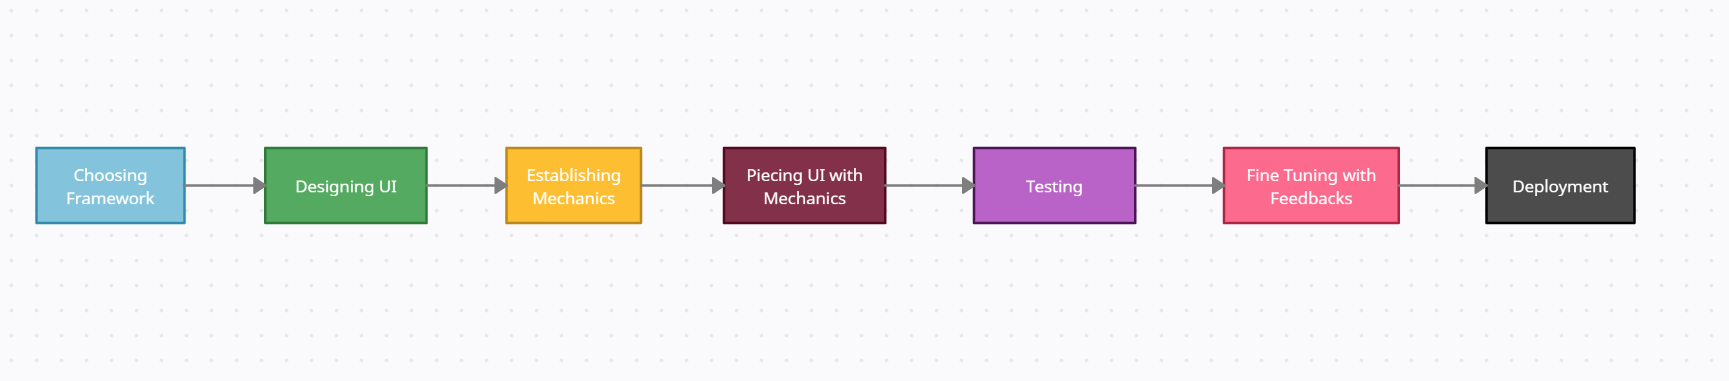
\includegraphics[scale=0.5]{SDLC.png}
\end{center}
\newpage

1.	Choosing Framework: The process of selecting a framework for our project was a crucial step, and we carefully evaluated different options before settling on Unity. We considered the ease of adoption, the quality of the documentation, and the level of community support for each engine.
2.	Designing UI: In terms of UI design, we were fortunate to have mentors with a keen sense of aesthetics who helped us create an interface that was both intuitive and visually appealing. We took great care to ensure that the UI complemented the gameplay mechanics and enhanced the user experience.

3.	Establishing Mechanics: Developing game mechanics that were accessible to players of all ages and skill levels was one of our primary goals. We spent a significant amount of time refining and simplifying the mechanics to ensure that they were easy to understand and provided a fun and engaging experience.

4.	Piecing UI with Mechanics: The mechanics were made in isolation and the UI designed differently since, we had to piece them together that really tells us the real story of development, fun and challenging at the same time. Integrating the UI and mechanics was a challenging but rewarding process. We designed them separately, which required us to carefully consider how they would work together and make the necessary adjustments to ensure that they were seamlessly integrated.

5.	Testing: Testing in gaming is a very strenuous job since there are many scopes to test with the available limited resources we have done Playtests, Network connection testing as well making sure there is no problem in mechanics and UI.Testing and quality assurance were critical components of our development process. We conducted extensive playtests, network connection testing, and comprehensive checks of mechanics and UI to ensure that the game was polished and free of bugs and glitches.

6.	Fine Tuning with Feedbacks: The edge and boundary cases of the game had a lot of bugs which led to backtracking our mistakes and making sure it was a tight ship. We encountered several bugs during the development process that required backtracking and debugging. We listened to feedback from players and continuously refined the game to ensure an optimal experience.

7.	Deployment: Deployment for a Unity cross platform has to be done across their own respective store so, for PC it is Steam or something for Apple their App Store and Android it is Google Play Store, since we are 4 students we chose to upload our game on itch.io for deployment and uploaded binaries for each platform, we chose itch.io since it is free and a lot of indie games are there already on it. Deploying a Unity cross-platform game requires uploading it to respective stores such as Steam for PC, Apple App Store for iOS, and Google Play Store for Android. As a team of four, we chose itch.io, a free platform that hosts many indie games, to upload our game. We uploaded binaries for each platform to itch.io.


%end of INtroduction



%start of Literature Survey
\centering
\section{LITERATURE SURVEY}


\justifying
\setlength{\parindent}{4em}
\setlength{\parskip}{0.5em}
\renewcommand{\baselinestretch}{1.5}
\normalsize
\begin{itemize}
\item \textbf STUDY OF RESEARCH PAPER
\end{itemize}
1.\textbf{Paper Name}:  An Emotional Recommender System for music [1]\\
\textbf{Author}:  Vincenzo Moscato, Antonio Picariello and Giancarlo Sperl´ [1]\\
\textbf{Description}: Recommender systems have become essential for users to find "what they need" 
in large collections of items. Meanwhile, recent studies have shown that user personality can 
effectively provide more valuable information to significantly improve the performance of 
recommenders, especially considering behavioral data captured from social network logs. In 
this work, they describe a new music recommendation technique based on the identification of 
personality traits, moods and emotions of a single user, based on solid psychological 
observations recognized by the analysis of user behavior in a social environment. In particular, 
users' personalities and moods have been incorporated into the content filtering approach to 
achieve more accurate and dynamic results.\\ 

\setlength{\parindent}{0em}
\textbf{2. Paper Name}:  Music Recommender System for users based on Emotion Detection through 
Facial Features [2]\\
\textbf{Author}:  Ahlam Alrihaili, Alaa Alsaedi, Kholood Albalawi [2].\\
\textbf{Description}:Facial emotion detection has received tremendous attention due to its 
applications in computer vision and human-computer interaction. In this research, they 
propose an emotion recognition recommendation system that is able to detect the user's 
emotions and suggest a list of suitable songs that can improve his mood. A short search was 
done on how music can affect a user's mood in the short term to gain knowledge and allow us 
to provide users with a list of music tracks that work well to improve the user's mood. The 
proposed system detects emotions, if the subject has a negative emotion, then he will be 
presented with a specific playlist containing the most suitable types of music that will improve 
his mood. On the other hand, if the detected emotion is positive, an appropriate playlist will 
be provided that will include different types of music that will enhance the positive emotion. 
The proposed recommendation system is implemented using the Viola-Jonze algorithm and 
PCA (Principal Component Analysis) techniques.\\

\setlength{\parindent}{0em}
\textbf{3. Paper Name}:  Emotional Detection and Music Recommendation System based on User
Facial Expression.[3]\\
\textbf{Author}: S Metilda Florence, M Uma [3]\\
\textbf{Description}:  Music plays a significant role in improving and uplifting the mood. It is often 
confusing for a person to decide what music to listen to from the vast collection of existing 
options. Analyzing the user's facial expression/emotions can lead to an understanding of the 
user's current emotional or mental state. This work focuses on a system that suggests songs to 
users based on their emotional state. The user's image is captured using a web camera. A 
snapshot of the user is taken and then according to the user's mood/emotion, a suitable song 
from the user's playlist is displayed to match the user's request.\\

\setlength{\parindent}{0em}
\textbf{4. Paper Name}: Facial Expression Based Music Player [4]\\
\textbf{Author}: Sushmita G. Kamble, Asso. Prof. A. H. Kulkarni [4]\\
\textbf{Description}:The conventional way of playing music depending on a person's mood requires 
human interaction. The transition to computer vision technology will enable the automation of 
such a system. To achieve this goal, an algorithm is used to classify human expressions and 
play a music track according to the currently detected emotion. It reduces the effort and time 
required to manually search for a song from a list based on a person's current state of mind. A 
person's expressions are detected by extracting facial features using the PCA algorithm and 
the Euclidean Distance classifier. In this paper, they use an embedded camera that is used to 
capture a person's facial expressions, which reduces the system design cost compared to other 
methods.\\
\vspace{7 cm}

\setlength{\parindent}{0em}
\textbf{5. Paper Name}:  Music Recommendation System Using Facial Expression Recognition Using 
Machine Learning. [5]\\
\textbf{Author}: B. Nareen Sai, D. Sai. Vamshi, Piyush Pogakwar, V. Seetharama Rao, Y. 
Srinivasulu [5]\\
\textbf{Description}:  The study of human emotional responses to visual stimuli such as photographs 
and movies, known as visual sentiment analysis, has proven to be a fascinating and difficult 
problem. Attempts to understand high-level information from visual data. The development 
of powerful algorithms from computer vision is responsible for the success of current 
models. Most existing models attempt to overcome the problem by recommending either 
robust features or more sophisticated models. Key suggested inputs are mainly visual 
elements from the entire image or video. Local areas have received less attention, which we 
believe is important for people's emotional response to the whole picture. Image recognition 
is used to find people in photos, analyze their emotions, and play emotion-related tunes based 
on their feelings. This repository achieves this goal by leveraging Google's Vision services. 
Given an image, it would search for faces, identify them, draw a rectangle around them, and 
describe the emotions it found.
\clearpage
%end of litterature

% SOFTWARE REQUIREMENT SPECIFICATION
\centering
\section{SOFTWARE REQUIREMENT SPECIFICATION}
\raggedright
\subsection{INTRODUCTION}

\justifying
\setlength{\parindent}{4em}
\setlength{\parskip}{0.5em}
\renewcommand{\baselinestretch}{1.5}

\normalsize
\hspace{1.7cm}\subsubsection{Project Scope}
Recommendation is about extending listeners music universe beyond what they know and
like. It empowers listeners once they have exhausted all their songs/artists searchcapabilities
with further navigation celerity
% code to fig reffrence==[figure. \ref{Simple Cryptography Process}].
\hspace{1.7cm}\subsubsection{ Assumption and dependencies}
\textbf{Domain}: Machine Learning\\
\textbf{Input}: Users’ Face

\centering
\raggedright
\subsection{ FUNCTIONAL REQUIREMENT}

\justifying
\setlength{\parindent}{4em}
\setlength{\parskip}{0.5em}
\renewcommand{\baselinestretch}{1.5}

\normalsize Proposed system consists of 4 modules:
\begin{itemize}\item User Registration: Firstly, user need to register in the system.
\item Login: After successful registration, user can login into the system.
\item Feature point extraction: Feature points of each user’s face gets detected.
\item Feature correspondence matching: Matching of selected feature points across
various image frames in database and display playlist.

\end{itemize}
\centering
\raggedright
\subsection{ EXTERNAL INTERFACE REQUIREMENT}

\justifying
\setlength{\parindent}{4em}
\setlength{\parskip}{0.5em}
\renewcommand{\baselinestretch}{1.5}
\subsubsection{ User Interface}
\normalsize\begin{itemize}\item  Machine Learning Based Music Recommendation System Using Facial 
Expressions
\end{itemize}
\subsubsection{ Hardware Interfaces:}
\normalsize\begin{itemize}\item   Hardware: Intel i5 Processor
\item  Speed: 2.80 GHz
\item  RAM: 8GB
\item  Hard Disk: 64 GB
\item  KeyBoard: Standard Windows Keyboard
\end{itemize}
\subsubsection{ Software Interfaces:}
\normalsize\begin{itemize}\item    Operating System: Windows 10(64 Bit) and Above.

\item   IDE: Spyder
\item  Programming Language: Python version 3.7,3.8

\end{itemize}

\centering
\raggedright
\subsection{ NON-FUNCTIONAL REQUIREMENT}

\justifying
\setlength{\parindent}{4em}
\setlength{\parskip}{0.5em}
\renewcommand{\baselinestretch}{1.5}
\subsubsection{ Performance Requirements}
\normalsize\begin{itemize}\item  The performance of the functions and every module must be well. The quality of the 
camera should be well resolved.
\item  The application is designed in modules where errors can be detected easily. This makes 
it easier to install and update new functionality if required.
\end{itemize}
\subsubsection{ Safety Requirement}
\normalsize\begin{itemize}\item   The application is designed in modules where errors can be detected and fixedeasily.
This makes it easier to install and update new functionality if required.

\end{itemize}
\subsubsection{  Software Quality Attributes}

\normalsize\begin{itemize}\item    Our system has many quality attributes that are given below:

1. Adaptability: This system is adaptable by all users.

2. Availability: This system is freely available to all users. The availability ofthe system
is easy for everyone.

3. Maintainability: After the deployment of the project if any error occurs then itcan be
easily maintained by the software developer.

4. Reliability: The performance of the system is better which will increase the reliability
of the Software.

5. User Friendliness: Since, the system is a GUI application; the output generated is 
much user friendly in its behavior.

6. Integrity: Integrity refers to the extent to which access to system or data by
unauthorized persons can be controlled.

7. Security: Users are authenticated using many security phases so reliable security is 
provided.

8. Testability: The system will be tested considering all the aspects
\end{itemize}

\centering
\raggedright
\subsection{ SYSTEM REQUIREMENTS}

\justifying
\setlength{\parindent}{4em}
\setlength{\parskip}{0.5em}
\renewcommand{\baselinestretch}{1.5}
\subsubsection{ Database Requirements}
Browser for SQLite (DB4S) is a high quality, visual and open-source tool to create, design, and 
edit database files compatible with SQLite. DB4S is for users and developers who want to 
create, search, and edit databases. DB4S uses a familiar spreadsheet-like interface, and
complicated SQL commands do not have to be learned. Controls and wizards are available for
users to:

\normalsize\begin{itemize}\item   Create and compact database files. Create, define, modify and delete tables. Create,
define, and delete indexes. Browse, edit, add, and delete records, Search records.
\item  Import and export databases from/to SQLite dump files.
\item  Issue SQL queries and inspect the results.

\end{itemize}
\subsubsection{Software Requirements}


\normalsize\begin{itemize}\item   Anaconda Navigator: Anaconda Navigator is a desktop graphical user interface 
(GUI) included in Anaconda distribution that allows you to launch applications and 
easily manage anaconda packages, environments, and channels without using
command line commands.
\item Anaconda.org or in a local Anaconda Repository. It is available for Windows,
macOS, and Linux. In order to run, many scientific packages depend on specific
versions of other packages. Data scientists often use multiple versionsof many 
packages and use multiple environments to separate these different versions.
\item  The command-line program conda is both a package manager and an environment 
manager. This helps data scientists ensure that each version of each package has all
the dependencies it requires and works correctly.
\item  Navigator is an easy, point-and-click way to work with packages and environments 
without needing to type conda commands in a terminal window. You can use it to 
find the packages you want, install them in an environment, run the packages and
update them – all inside Navigator.

\end{itemize}
\subsubsection{Hardware Requirements}

\normalsize\begin{itemize}\item  RAM: 8 GB
As we are using Machine Learning Algorithm and Various High-Level Libraries
Laptop RAM minimum required is 8 GB.

\item Hard Disk: 64 GB
\item Processor: Intel i5 Processor

\end{itemize}
\centering
\raggedright
\subsection{  ANALYSIS MODELS: SDLC MODEL TO BE APPLIED}

\justifying
\setlength{\parindent}{4em}
\setlength{\parskip}{0.5em}
\renewcommand{\baselinestretch}{1.5}
\subsubsection{ User Interface}
\normalsize
SDLC Models stands for Software Development Life Cycle Models. In this report, we explore 
the most widely used SDLC methodologies such as Agile.Each software development life 
cycle modelstarts with the analysis. Also, here are defined the technologies used in the project.
One of the basic notions of the software development process is SDLC models which stands 
for Software Development Life Cycle models. SDLC – is a continuous process, which starts 
from the moment, when it’s made a decision to launch the project, and it ends at the moment 
of its full remove from the exploitation. There is no one single SDLC model. They are divided 
into maingroups, each with its features and weaknesses

\begin{itemize}\item Requirement gathering and analysis: In this step, we identify what are various 
requirements are needed for our project such are software and hardware required, 
database, and interfaces.

\item System Design: In design phase we design the system which iseasily understood for 
end user i.e., user friendly. We design some UML diagrams and data flow diagram to 
understand the system flow and system module and sequence of execution.

\item Implementation: In implementation phase of our project, we will implement various 
module required for successfully getting expected outcome at the different module 
levels. With inputs from system design, the system is first developed in small programs
called units, which are integrated in the nextphase. Each unit is developed and tested
for its functionality which is referred to as Unit Testing.

\item Testing: The different test cases are performed to test whether the project module is
giving expected outcome in assumed time. All the units developed in the
implementation phase are integrated into a system after testing of each unit. Post 
integration the entire system is tested for any faults and failures.

\item Deployment of System: Once the functional and non-functional testing is done, the
product is deployed in the customer environment or released into the market

\item Maintenance: There are some issues which come up in the client environment. To fix 
those issues patches are released. Also, to enhance the product some better versions are 
released. Maintenance is done to deliver these changes in the customer environment. All 
these phases are cascaded to each other in which progress is seen as flowing steadily 
downwards like a waterfall through the phases. The next phase isstarted only after the 
defined set of goals are achieved for previous phase and it is signed off.



\end{itemize}
\centering
\raggedright
\subsubsection{Project Resource}
Well configured Laptop, Anaconda Navigator, 64 GB RAM.
\clearpage
\centering
\raggedright
\subsection{ SDLC MODEL}
\vspace{2cm}
\begin{figure}[h]
\centering
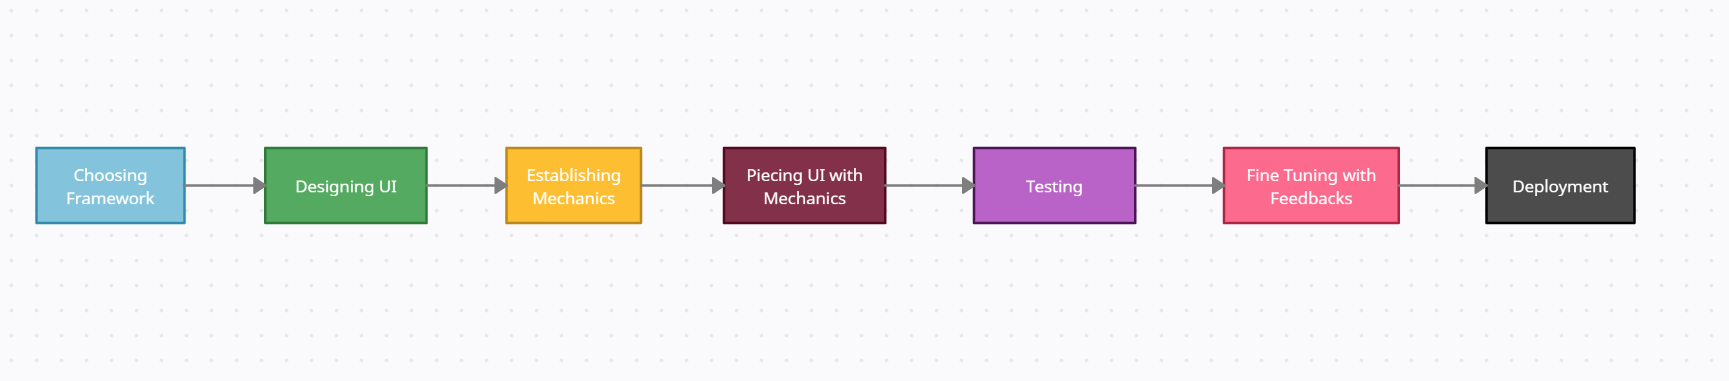
\includegraphics[scale=0.9]{SDLC.png}
\caption{SDLC MODEL}
\label{SDLC}
\end{figure}
\clearpage
% end of SRS

%  SYSTEM DESIGN

\centering
\section{ SYSTEM DESIGN}
\raggedright
\subsection{SYSTEM ARCHITECTURE}

\justifying
\setlength{\parindent}{4em}
\setlength{\parskip}{0.5em}
\renewcommand{\baselinestretch}{1.5}

\vspace{0.5cm}
\begin{figure}[h]
\centering
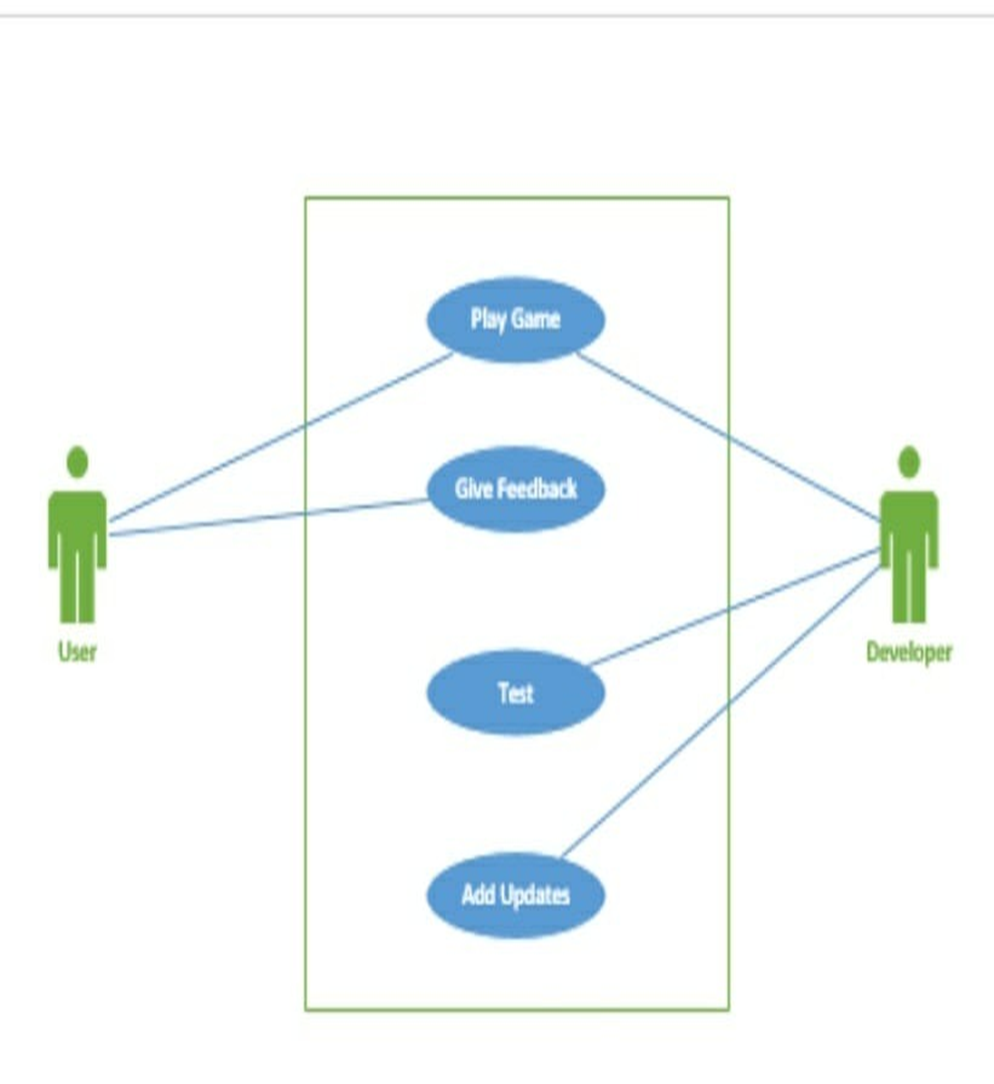
\includegraphics[scale=0.7]{Architecture.png}
\caption{ System Architecture}
\label{ System Architecture}
\end{figure}
\vspace{0.1cm}
\subsubsection{Explanation}
\hspace{1.7cm}Steps involved to design the system, training dataset and test images are considered for 
which the following procedures are applied to get the desired results. The training set is 
the data which has large amount of data stored in it and the test set is the input given for
recognition purpose.\\
\hspace{1.7 cm} The whole system is designed in 5 steps:

\textbf{1. Image Acquisition:} In any of the image processing techniques, the first task is to 
acquire the image from the source. These images can be acquired either through
camera. The images considered here are user dependent i.e., dynamic images.

\textbf{2. Pre-processing: } Pre-processing is mainly done to eliminate the unwanted information
from the image acquired and fix some values for it, so that the value remains same 
throughout. During pre-processing, eyes, nose and mouth are considered to be the region of
interest. It is detected by the cascade object detector which utilizes Haar Cascade
Feature.



\textbf{ 3. Facial Feature Extraction:}After pre-processing, the next step is feature extraction. 
The extracted facial features are stored as the useful information during training phase 
and testing phase. The following facial features canbe considered ―Mouth, forehead,
eyes, cheek and chin dimple, eyebrows, nose and wrinkles on the face‖. In this work, 
eyes, nose, mouth and fore-head are considered for feature extraction purpose for the
reason that these depict the most appealing expressions.With the wrinkles on the 
forehead or the mouth being opened one can easily recognize that the person is either 
surprised or is fearful. But with a person’s complexion it can never be depicted. To 
extract the facial features Haar feature technique is used.

\textbf{4. Expression Recognition:} To recognize and classify the expressions of a person
Convolution Neural Network. classifier is used. It gets the nearest match for the test data 
from the training data set and hence gives a better match for the current expression 
detected.Face detection is a non-trivial computer vision problem for identifying and 
localizing faces in images. Face detection can be achieved using 
a Multi-task Cascade CNN.


\textbf{5. Play Music:} The last and the most important part of this system is the playing of music
based on the current emotion detected of an individual. Once the facial expression of the 
user is classified, the user’s corresponding emotional state is recognized. Severalsongs
from various domains pertaining to a number of emotions is collected and put up in the 
list. Each emotion category has a number of songs listed in it. When the user’s
expression is classified with the help of CNN algorithm, songs belonging to that 
category are then played.
%end of design


\clearpage
%  start ALGORITHM
\centering
\section{ALGORITHM}

\justifying
\setlength{\parindent}{4em}
\setlength{\parskip}{0.5em}
\renewcommand{\baselinestretch}{1.5}
\normalsize
\subsection{ Convolutional Neural Networks (CNN):}
\hspace{1.7cm} Convolutional Neural Networks, a type of deep learning algorithm, are very good at analyzing 
images. Best algorithm for automatic processing of images. The image contains RGB 
combination data. You can use matplotlib to import an image from a file into memory. A 
convolutional neural network is a special type of neural network that helps machines learn and 
classify images. 

A convolutional neural network has three types of layers:

1) Convolutional Layer: Each input neuron in a typical neural network is connected to the 
following hidden layer. Only a small fraction of the CNN’s input layer neurons are connected 
to the hidden layer of neurons.

2) Pooling Layer: The dimensionality of the feature map is reduced using a pooling layer. 
Within the hidden layers of a CNN, there are many activation and pooling layers.

3) Fully-Connected layer: The last few layers of the network are known as fully connected 
layers. The output of the final pooling or convolutional layer is fed to the fully connected 
layer and flattened before being applied.

%\begin{figure}[h]
%\centering
%\includegraphics[scale=0.6]{CNN Algorithm.png}
%\caption{CNN Algorithm}
%\label{CNN Algorithm}
%\end{figure}



\subsection{ Haar Cascade Feature}
\hspace{1.7cm}This is an object detection algorithm used to identify faces in real-time images or videos. 
This algorithm uses the edge or line detection feature proposed by Viola and Jones in year 
2001 research paper, “Rapid Object Detection using a Boosted Cascade of Simple 
Features”. This algorithm contains many positive image planes and many negative images 
that have not been added.
\vspace{1.5cm}
\begin{figure}[h]
\centering
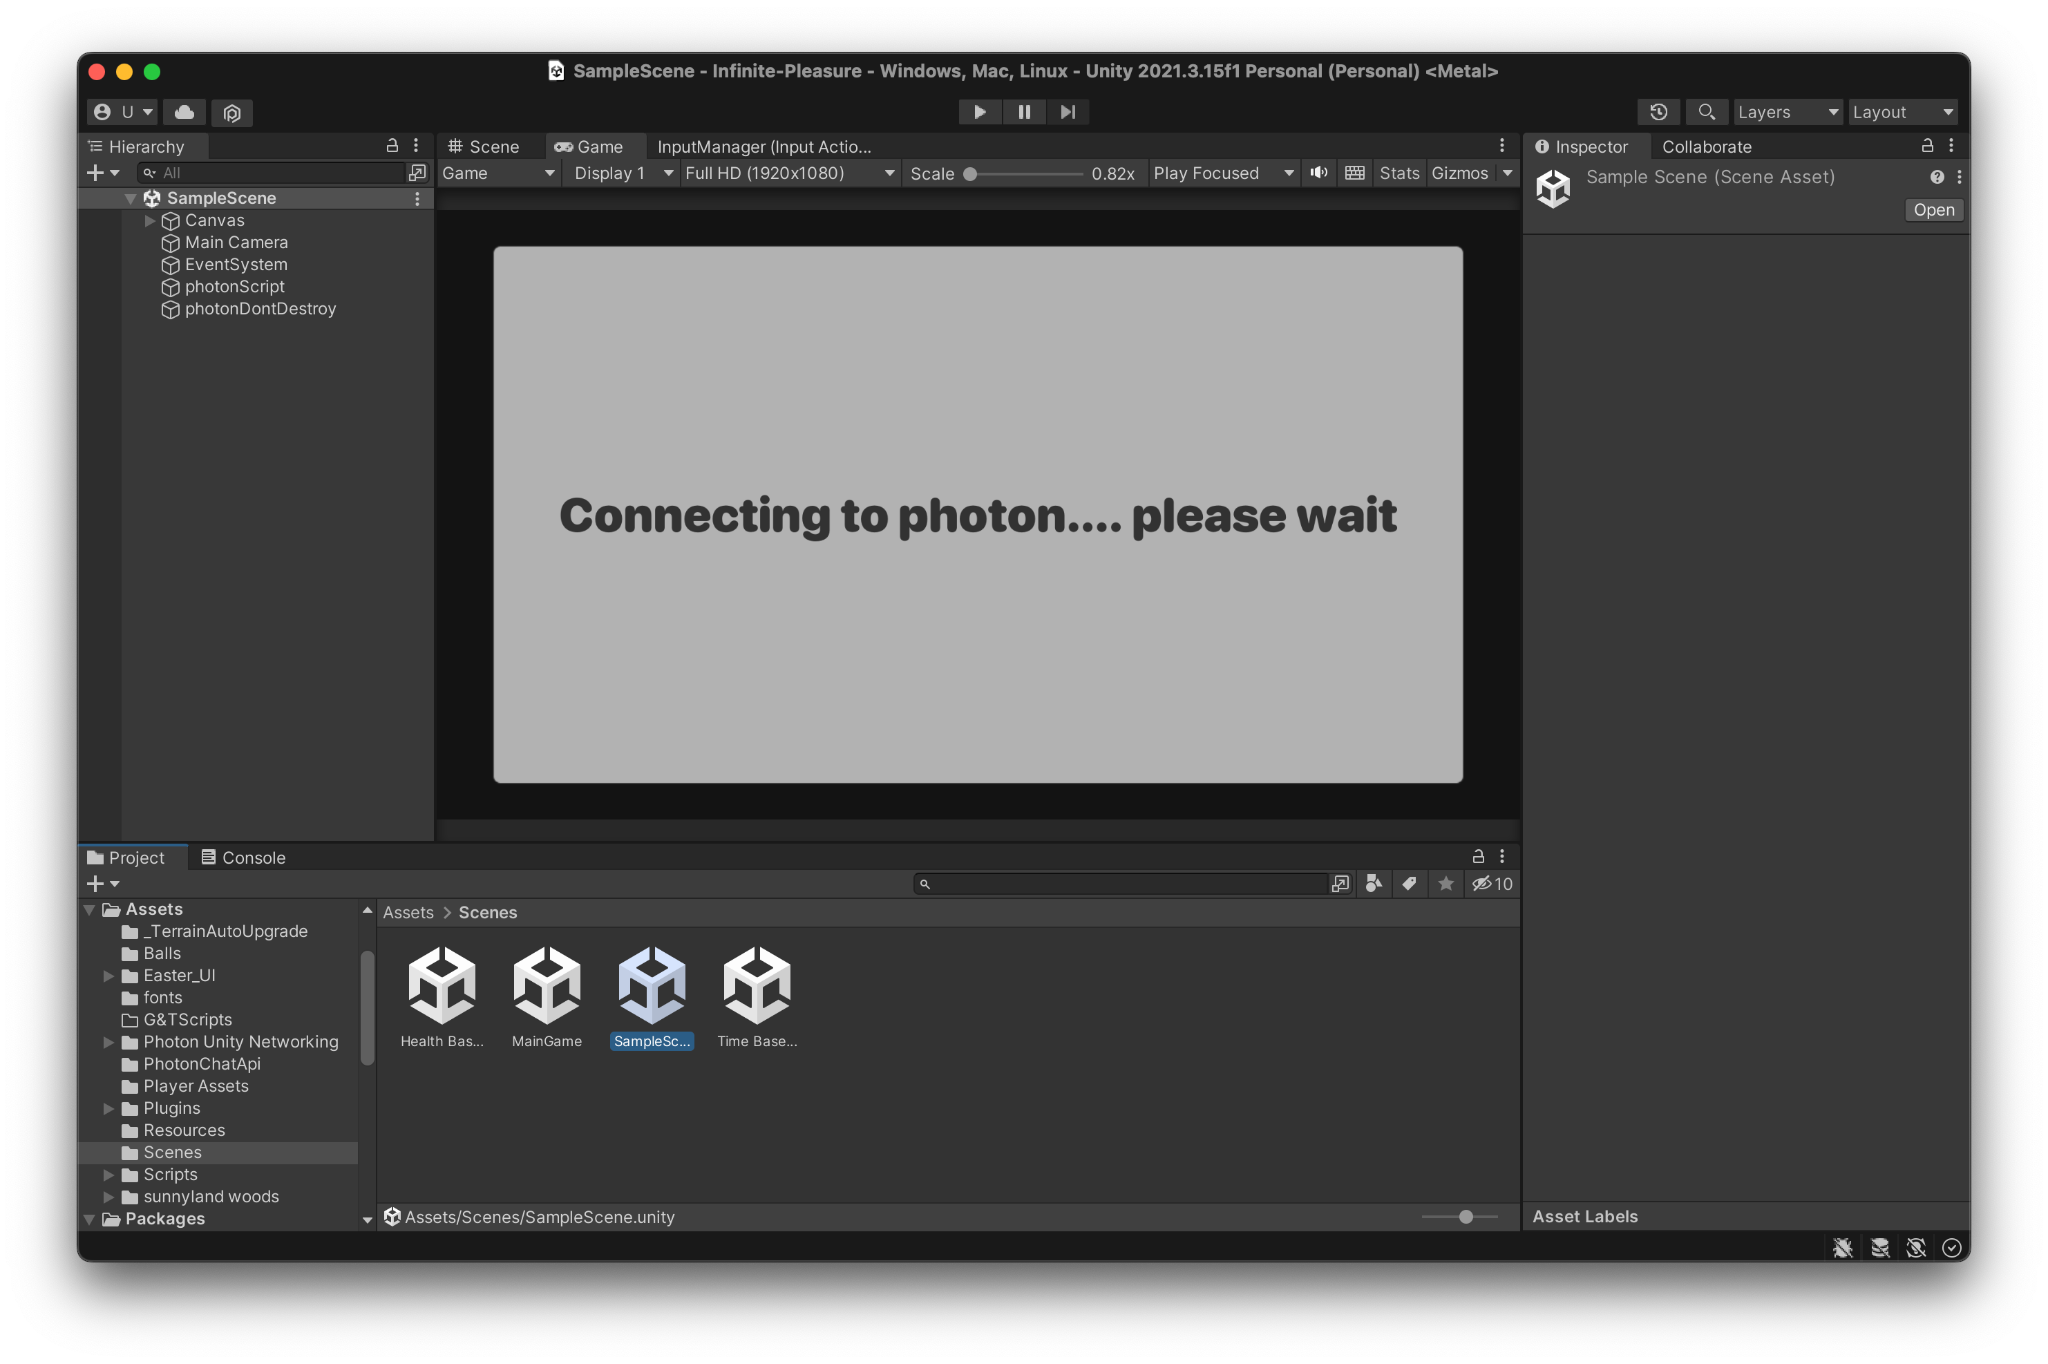
\includegraphics[scale=0.6]{Haar.png}
\caption{Haar Cascade Feature}
\label{Haar Cascade Feature}
\end{figure}
\clearpage

\vspace{4cm}
\raggedright
\centering
\section{DIAGRAMS}
\justifying
\setlength{\parindent}{4em}
\setlength{\parskip}{0.5em}
\renewcommand{\baselinestretch}{1.5}
\normalsize
\subsection{Data Flow Diagram}
In Data Flow Diagram, we Show that flow of data in our system in DFD0 we show that 
base DFD in which rectangle present input as well as output and circle show our system. 
In DFD1 we show actual input and actual output of system input of our system is text or 
image and output is rumor detected likewise in DFD 2 we presentoperation of user as well
as admin.

\vspace{1cm}
\begin{figure}[h]
\centering
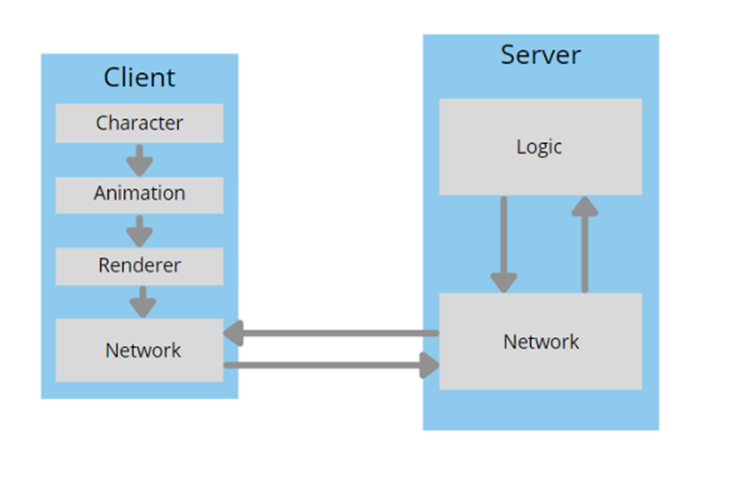
\includegraphics[scale=0.7]{ Data Flow diagram-0.png}
\caption{ Data Flow diagram-0}
\label{ Data Flow diagram-0}
\end{figure}


\vspace{1cm}
\begin{figure}[h]
\centering
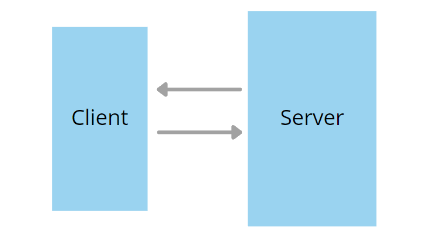
\includegraphics[scale=0.8]{ Data Flow diagram-1.png}
\caption{ Data Flow diagram-1}
\label{ Data Flow diagram-1}
\end{figure}



\vspace{1.5cm}
\begin{figure}[h]
\centering
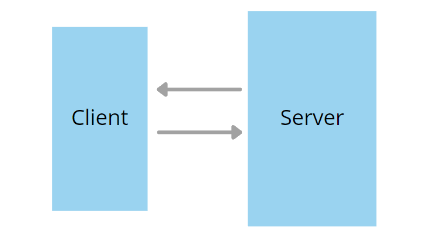
\includegraphics[scale=1.0]{ Data Flow diagram-1.png}
\caption{ Data Flow diagram-2}
\label{ Data Flow diagram-2}
\end{figure}


\clearpage
\justifying
\setlength{\parindent}{4em}
\setlength{\parskip}{0.5em}
\renewcommand{\baselinestretch}{1.5}
\normalsize
\subsection{UML DIAGRAMS}
Unified Modeling Language is a standard language for writing software blueprints. The
UML may be used to visualize, specify, construct and document the artifacts of a soft- ware
intensive system. UML is process independent, although optimally it should be used in
process that is use case driven, architecture centric, iterative and incremental. The Number
of UML Diagram is available.


\begin{itemize}
\item Use case Diagram.

\item Component Diagram.

\item Activity Diagram

\item  Sequence Diagram.

\end{itemize}

\clearpage


\justifying
\setlength{\parindent}{4em}
\setlength{\parskip}{0.5em}
\renewcommand{\baselinestretch}{1.5}
\normalsize
\subsection{Use Case Diagram}
A use case diagram in the Unified Modelling Language (UML) is a type of behavioral
diagram defined by and created from a Use-case analysis. Its purpose is to present a graphical 
overview of the functionality provided by a system in terms of actors, their goals 
(represented as use cases), and any dependencies between those use cases. The main purpose 
of a use case diagram is to show what system functions are performed for which actor. Roles 
of the actors in the system can be depicted.


\vspace{1.5cm}
\begin{figure}[h]
\centering
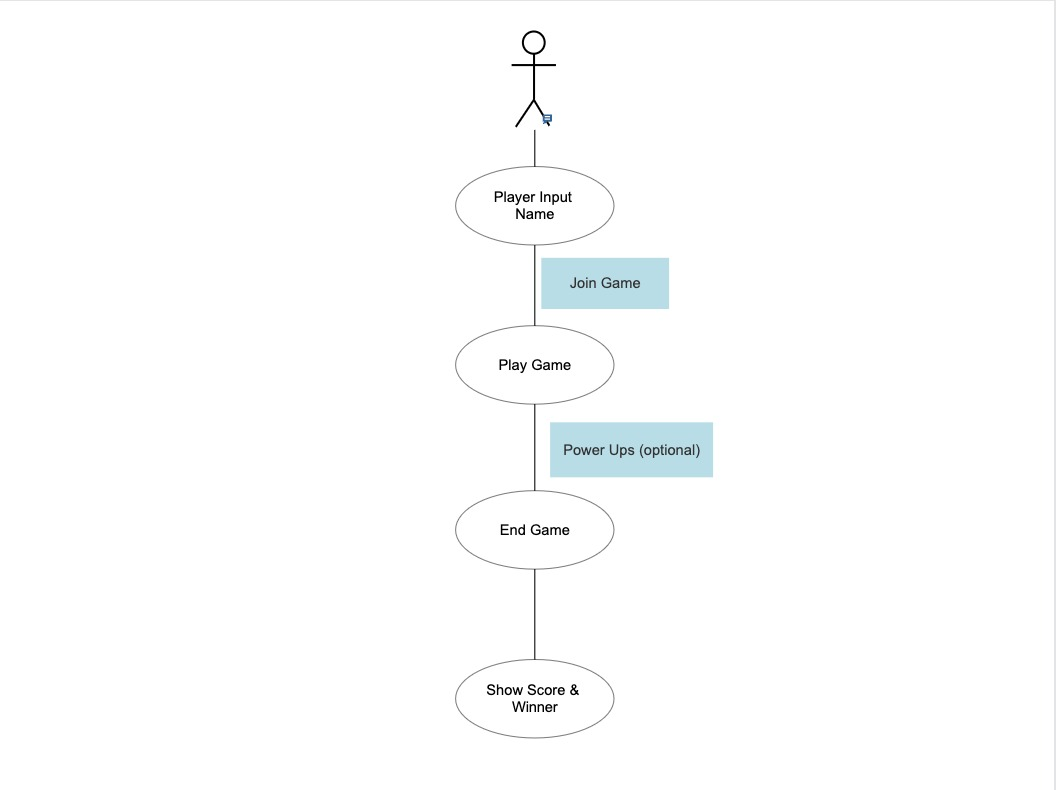
\includegraphics[scale=0.7]{images15.png}
\caption{Use case Diagram}
\label{ Use case Diagram}
\end{figure}

\justifying
\setlength{\parindent}{4em}
\setlength{\parskip}{0.5em}
\renewcommand{\baselinestretch}{1.5}
\normalsize
\subsection{Activity Diagram}
An activity is particular operation of the system. An activity diagram is intended to represent
stepwise work-flow of activities or actions that can take place in the system. It shows overall
flow of control and models computational and organizational processes. Activity diagrams
are used to model dynamic aspects of the system. 

\vspace{1.5cm}
\begin{figure}[h]
\centering
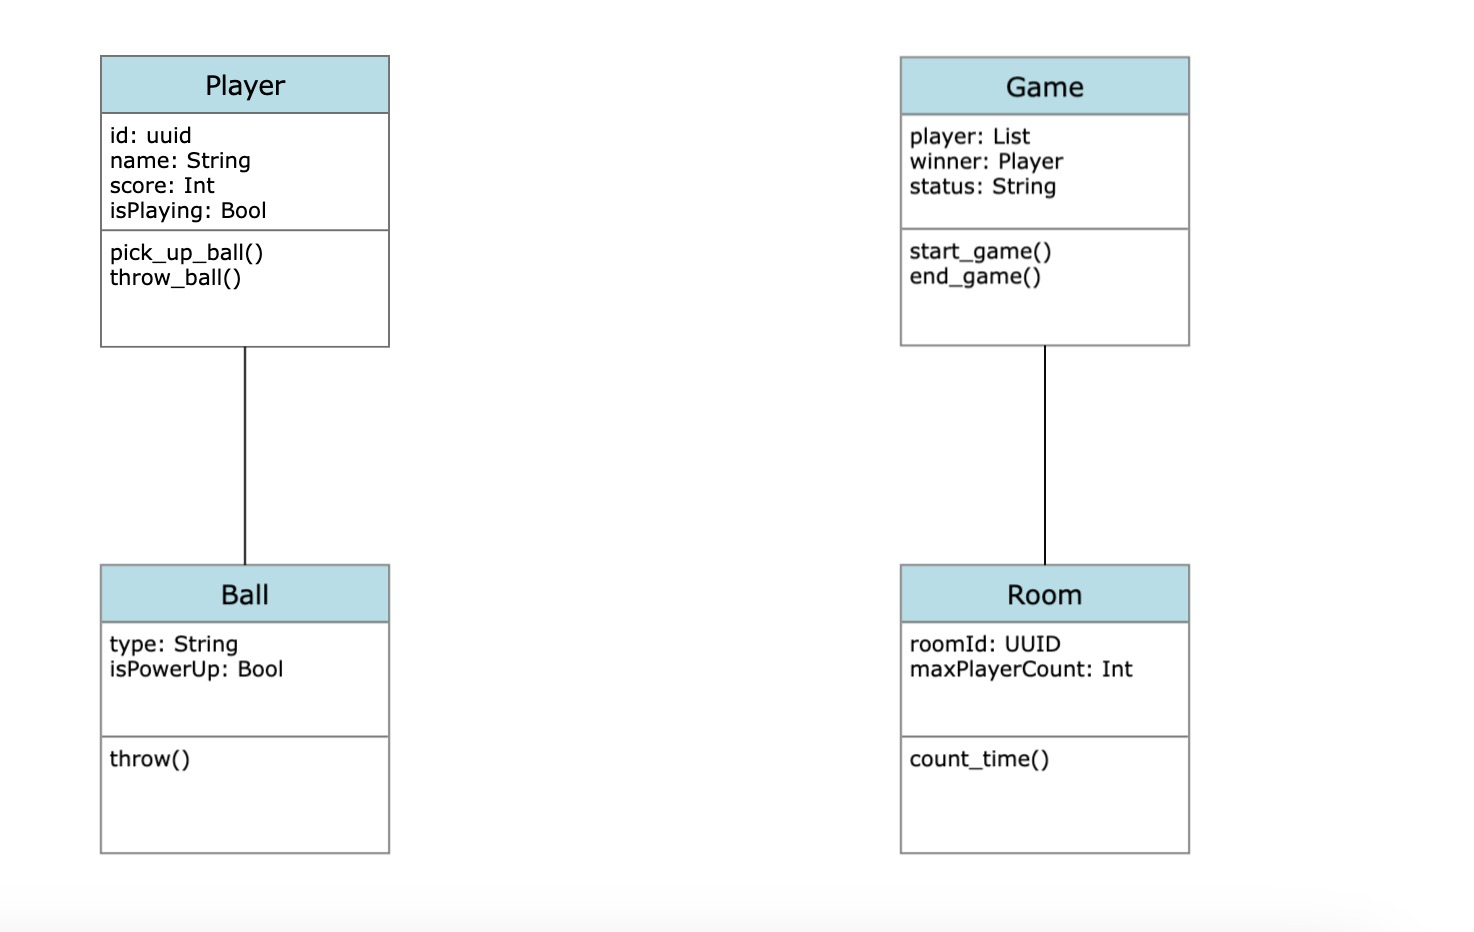
\includegraphics[scale=0.8]{images14.png}
\caption{Activity Diagram}
\label{Activity Diagram}
\end{figure}


\justifying
\setlength{\parindent}{4em}
\setlength{\parskip}{0.5em}
\renewcommand{\baselinestretch}{1.5}
\normalsize
\subsection{Sequence Diagram}
Sequence diagram shows how objects communicate with each other in terms of a sequence 
of messages. It also indicates the lifespans of objects relative to those messages.
\vspace{1.5cm}
\begin{figure}[h]
\centering
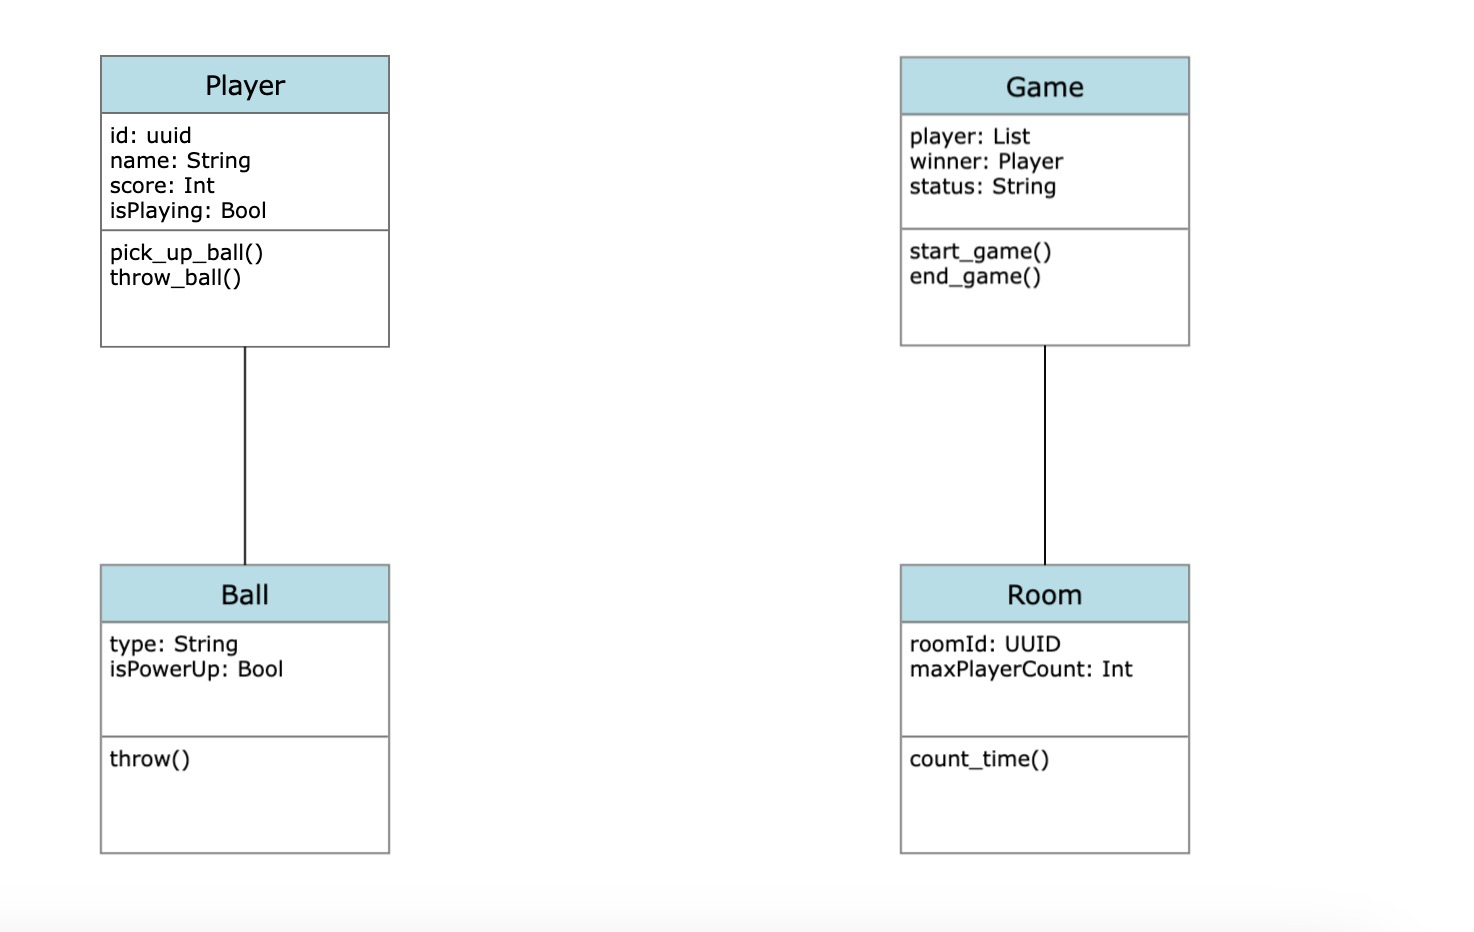
\includegraphics[scale=0.9]{images14.png}
\caption{Sequence Diagram}
\label{Sequence Diagram}
\end{figure}

\clearpage
\justifying
\setlength{\parindent}{4em}
\setlength{\parskip}{0.5em}
\renewcommand{\baselinestretch}{1.5}
\normalsize
\subsection{ Class Diagram}
Class diagram describes the structure of a system by showing the system’s classes, Their
attributes, and the relationships among the classes. Proposed system contains five different 
types of classes and each posses their own attributes and methods. Main Classes of the 
proposed system are NDSRRC, FP Tree, Apriory, Sanitised DB each have different 
functionalities.
\vspace{1.5cm}
\begin{figure}[h]
\centering
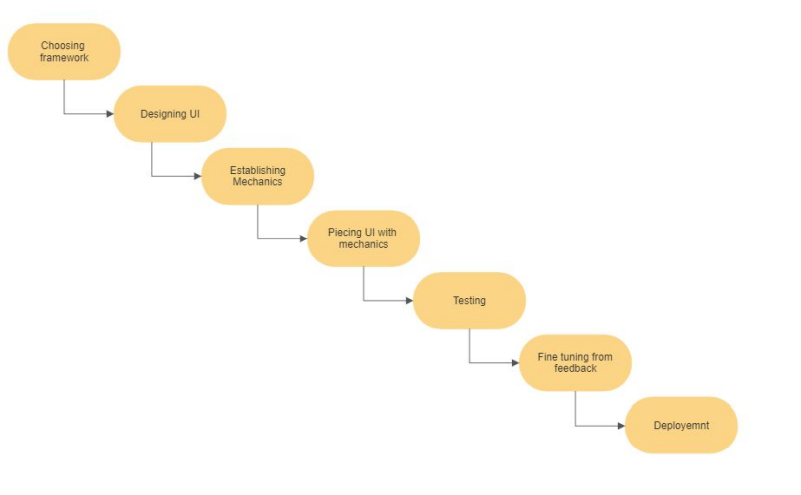
\includegraphics[scale=0.9]{ Class Diagram.png}
\caption{ Class Diagram
}
\label{ Class Diagram
}
\end{figure}


\clearpage
\justifying
\setlength{\parindent}{4em}
\setlength{\parskip}{0.5em}
\renewcommand{\baselinestretch}{1.5}
\normalsize
\subsection{ Entity Relationship Diagrams}
Class diagram describes the structure of a system by showing the system’s classes, Their
attributes, and the relationships among the classes. Proposed system contains five different 
types of classes and each posses their own attributes and methods. Main Classes of the 
proposed system are NDSRRC, FP Tree, Apriory, Sanitised DB each have different 
functionalities.
\vspace{1.5cm}

\clearpage
\centering
\section{ Project Estimation and Project Plan}
\justifying
\setlength{\parindent}{4em}
\setlength{\parskip}{0.5em}
\renewcommand{\baselinestretch}{1.5}
\normalsize In this chapter we are going to have an overview about how much time does it took to complete each task like- Preliminary Survey Introduction and Problem Statement, Literature Survey, Project Statement, Software Requirement and Specification, System Design, Partial Report Submission, Architecture Design, Implementation, Deployment, Testing, Paper Publish, Report Sub- mission and etcetera. This chapter also focuses on the stakeholder list which gives information about project type, customer of the proposed system, user and project member who developed the system.

\subsection{PROJECT ESTIMATES}
\large\textbf{MATHEMATIC MODEL}
\justifying
\setlength{\parindent}{4em}
\setlength{\parskip}{0.5em}
\renewcommand{\baselinestretch}{1.5}
\vspace{0.1cm}
\begin{enumerate}
\item Let S be the system that detects Sample Space\\
S= {.......}


\item  Identify input as I\\
S= {I....}\\
I= {Vi — where vi is input transactional DB from user}

\item  Identify output as O\\
S= {I, O, ...}\\
O= {Vo — where Vo is sanitized DB for given DB by user}

\item  Identify the Processes as P\\
S= {I, O, P, ...}\\
P= {BN, DB, CS, A, HS}
\begin{itemize}
\item  BN as Binarization
\item DB as derive association rule from DB
\item CS as Calculate sensitive rules
\item A as Analyze sensitivity of the RHS of element
\item HS hide the sensitive rule
\end{itemize}

\item Identify the failure case F\\
S= {I, O, P, F, ...}\\
F= {failure occurs when a sensitive rule remains visible}

\item  Identify the success case s\\
S= {I, O, P, F, s, …}\\
s= {success means when a correct sensitive rule is identified and get hide}

\item Identify the initial condition\\
S= {I, O, P, F, s, IC}\\
IC= {Initial condition is that DB in transactional DB} 

\end{enumerate}

\subsection{RISK MANAGEMENT}
\justifying
\setlength{\parindent}{4em}
\setlength{\parskip}{0.5em}
\renewcommand{\baselinestretch}{1.5}
\vspace{0.1cm}
\begin{enumerate}
\item In appropriate dataset -To overcome this risk we are trying to use a well organized and complete dataset.
\item Security- To overcome and improve security we use multilevel security like access permissions of users.

\end{enumerate}
\subsubsection{Risk Identification}
\justifying
\setlength{\parindent}{4em}
\setlength{\parskip}{0.5em}
\renewcommand{\baselinestretch}{1.5}
\vspace{0.1cm}
\begin{enumerate}
\item Are end-users enthusiastically committed to the project and the sys- tem/product to be built?
Ans-Not known at this time.
\item Are requirements fully understood by the software engineering team and its customers?
Ans-Yes
\item Does the software engineering team have the right mix of skills? Ans-yes
\item Is the number of people on the project team adequate to do the job? Ans-Not applicable
\item Do all customer/user constituencies agree on the importance of the project and on the requirements for the system/product to be built?
Ans-Not applicable
\end{enumerate}


\subsubsection{Risk Analysis}
\justifying
\setlength{\parindent}{4em}
\setlength{\parskip}{0.5em}
\renewcommand{\baselinestretch}{1.5}
\vspace{0.1cm}
\normalsize
The risks for the Project can be analyzed within the constraints of time and quality.Risk analysis for a malware detection system using SVM involves assessing potential vulnerabilities, threats, and potential impacts. Here's an overview of the risk analysis process:
\begin{itemize}
\item \textbf{Identify system vulnerabilities:} Identify the vulnerabilities in the malware detection system that could be exploited by attackers. This could include weaknesses in the SVM implementation, data storage, network communication, or any other component of the system.
\item \textbf{Threat identification:}: Identify potential threats that the system may face. This can include external threats, such as attackers attempting to bypass the detection system or exploit vulnerabilities, as well as internal threats, such as insider attacks or unintentional misuse of the system.
\item \textbf{Impact assessment: } Evaluate the potential impact of a successful attack or system failure. Consider the consequences in terms of data compromise, system downtime, financial losses, reputational damage, or any other relevant factors. This step helps prioritize risks based on their potential impact.
\item \textbf{Risk evaluation:} Combine the impact and likelihood assessments to determine the level of risk associated with each identified threat. This can be done by assigning risk levels, such as low, medium, or high, or by using a numerical risk scoring system. This step helps prioritize risks for mitigation efforts.
\item \textbf{Risk mitigation :}Develop strategies and measures to mitigate the identified risks. This may include implementing security controls, applying patches and updates, enhancing system monitoring and logging, conducting regular security assessments, or training system users to minimize human errors.
\item \textbf{Monitoring and review:} Regularly monitor the malware detection system and review the effectiveness of implemented risk mitigation measures. Stay updated on the evolving threat landscape and adjust risk mitigation strategies accordingly.
It's important to note that risk analysis should be an ongoing process, continuously adapted to address emerging threats and changes in the system and its environment. Regular risk assessments and updates to the malware detection system are essential to maintain a robust security posture.

\end{itemize}
\vspace{14cm}
\subsubsection{Risk Mitigation Risk Monitoring and Risk Management}
\justifying
\setlength{\parindent}{4em}
\setlength{\parskip}{0.5em}
\renewcommand{\baselinestretch}{1.5}

\normalsize
\vspace{1cm}

\vspace{14cm}
\subsection{PROJECT SCHEDULE}

\justifying
\setlength{\parindent}{4em}
\setlength{\parskip}{0.5em}
\renewcommand{\baselinestretch}{1.5}
\subsubsection{Project Task Set}
\normalsize
Major Tasks in the Project stages are:
\begin{enumerate}
\item Task 1: correctness
\item Task 2: availability
\item Task 3: integrity
\end{enumerate}
\vspace{0.1cm}


\vspace{14cm}
\subsection{Timeline Chart}
\justifying
\setlength{\parindent}{4em}
\setlength{\parskip}{0.5em}
\renewcommand{\baselinestretch}{1.5}

\vspace{1cm}











\clearpage


\centering
\section{OTHER SPECIFICATION}

\justifying
\setlength{\parindent}{4em}
\setlength{\parskip}{0.5em}
\renewcommand{\baselinestretch}{1.5}

\vspace{0.5cm}
\normalsize
\subsection{  ADVANTAGES}
\begin{itemize}
\item The main advantage of our music recommendation system is to provide 
suggestions to the users that fit the user's emotions.\\
\item The analysis of the facial expression/user emotion may lead to understanding the 
current emotional state of the user
\end{itemize}

\vspace{1.5cm}
\normalsize
\subsection{  APPLICATIONS}
\begin{itemize}
\item This system helps user to play songs automatically according to their mood.\\
\item Redirection of page to the music website once song is played.

\end{itemize}
\clearpage

\centering
\section{RESULT}

\justifying
\setlength{\parindent}{4em}
\setlength{\parskip}{0.5em}
\renewcommand{\baselinestretch}{1.5}
\vspace{1cm}



\vspace{1cm}


\vspace{1.5cm}


\vspace{1cm}


\vspace{1.5cm}


\vspace{1cm}


\vspace{1cm}


\vspace{1.5cm}


\vspace{1cm}

\clearpage
\centering
\section{TESTING}
\justifying
\setlength{\parindent}{4em}
\setlength{\parskip}{0.5em}
\renewcommand{\baselinestretch}{1.5}
\normalsize
\subsection{ Introduction}
\hspace{1.7 cm}Testing is an important part of software development life cycle. It is performed to ensure 
quality of the developed system. Testing includes a set of investigative activities that can be 
planned in advance and conducted systematically, to assure the stakeholder that system 
fulfils all the requirements gathered during requirement gathering phase. Software testing is 
one of the key elements in software projects that is often referred to as verification and 
validation. Verification refers to the set of activities that ensure that software correctly 
implements specified functionality. Validation refers to a set of activities built around 
traceability matrix which ensure that the functionality implemented by the system is 
traceable to customer requirements

Tests are the individual tests specified in a test plan document. Each test is typically 
described by
\begin{itemize}
\item An initial system state.
\item A set of actions to be performed.
\item The expected results of the test.
\end{itemize}

\subsection{ Implementation}
\justifying
\setlength{\parindent}{4em}
\setlength{\parskip}{0.5em}
\renewcommand{\baselinestretch}{1.5}
\normalsize

Test cases are planned in accordance to the test process and documented with detailed test 
descriptions. These test cases use cases based on projected operational mission scenarios. 
The testing process also includes stress or load testing for stability purpose (i.e., at 95% CPU 
use, system stability is still guaranteed. The test process thoroughly tests the interfaces and 
modules. Software testing includes a traceable white box testing, black box testing and other 
test processes verifying implemented software against design documentation and 
requirements specified.


\subsection{Objective
}
\justifying
\setlength{\parindent}{4em}
\setlength{\parskip}{0.5em}
\renewcommand{\baselinestretch}{1.5}
\normalsize

The software test plan (STP) is designed to test each module to measure its performance, to 
uncover bugs in the system, to set aright any flaws in logic that may be present, and to check 
logical flow from one module to another within system.
\begin{itemize}
\item All field entries must work properly.
\item Pages must be activated from the identified link.
\item The entry screen, messages and responses must not be delayed.

\end {itemize}


\subsection{Testing Strategy
}
\justifying
\setlength{\parindent}{4em}
\setlength{\parskip}{0.5em}
\renewcommand{\baselinestretch}{1.5}
\normalsize

A strategy outlines what to plan, and how to plan it. A successful strategy is your guide 
through change, and provides a firm foundation for ongoing improvement. Unlike a plan, 
which is obsolete from the point of creation, a strategy reflects the values of an organization 
- and remains current and useful. When an organization tests its products or its tools, it tries 
to compare them against its expectations and values. By its nature, testing introduces change 
as problems are identified and resolved. A test strategy is necessary to allow these two 
impulses to work together. Furthermore, testing can never be said to be ‘complete’, and a 
core skill in testing is the justified management of conflicting demands; without a strategy, 
these judgements will be inconsistent to the point of failure.\\
Software development is a creative process. A test strategy is a vital enabler to this process 
keeping focus on core values and consistent decision-making to help achieve desired goals 
with best use of resource. 

\subsection{ Types of Testing:
}
\justifying
\setlength{\parindent}{4em}
\setlength{\parskip}{0.5em}
\renewcommand{\baselinestretch}{1.5}
\normalsize

\hspace{1.7 cm} 1. White Box Testing: A level of white box test coverage is specified that is ap propriate for 
the software being tested. The white box and other testing uses automated tools to instrument 
the software to measure test coverage.

2. Black Box Testing: A black box test of integration builds includes functional, interface, 
error recovery, stress and out-of-bounds input testing. All black box software tests are traced 
to control requirements. In addition to static requirements, a black box of a fully integrated 
system against scenario sequences of events is designed to model field operation. 
Performance testing for systems is integrated as an integral part of the black box test process.


\subsection{ Unit Testing
}
\justifying
\setlength{\parindent}{4em}
\setlength{\parskip}{0.5em}
\renewcommand{\baselinestretch}{1.5}
\normalsize

Unit testing is used to check the execution path of the module, function, and procedure of 
the system. Test is conducted with the help of normal data and abnormal data. This testing 
includes the different factors like statement coverage, branch coverage, loop processing, 
abnormality, and circulation etc. With the help of this Unit testing we check that all the 
statement in the code is executed or not so it avoids the dead code statement. It checks all 
the branches and execution path of the code. It ensures that all the internal method of 
program are executed and properly integrated with program.

Unit testing involves the design of test cases that validate that the internal program logic is 
functioning properly, and that program inputs produce valid outputs. All decision branches 
and internal code flow should be validated. It is the testing of individual software units of 
the application .it is done after the completion of an individual unit before integration. This 
is a structural testing, that relies on knowledge of its construction and is invasive. Unit tests 
perform basic tests at component level and test a specific business process, application, 
and/or system configuration. Unit tests ensure that each unique path of a business process 
performs accurately to the documented specifications and contains clearly defined inputs 
and expected results.

\subsection{Integrated system}
\justifying
\setlength{\parindent}{4em}
\setlength{\parskip}{0.5em}
\renewcommand{\baselinestretch}{1.5}
\normalsize

In integrated testing, all the modules are checked together to ensure that all the modules are 
executing together according to the program specification. Once all the mod ules have been 
tested individually, the most legitimate question can be asked is that when all the modules 
are working properly, why there is need of integrated testing.

The answer is, though all modules are working properly problem may occur while interfacing 
individual module. Testing is event driven and is more concerned with the 
basic outcome of screens or fields. Integration tests demonstrate that although the components 
were individually satisfaction, as shown by successfully unit testing, the combination of 
components is correct and consistent. Integration testing is specifically aimed at exposing the 
problems that arise from the combination of components.

\subsection{ Functional test}
\justifying
\setlength{\parindent}{4em}
\setlength{\parskip}{0.5em}
\renewcommand{\baselinestretch}{1.5}
\normalsize

Functional tests provide systematic demonstrations that functions tested are available as 
specified by the business and technical requirements, system documentation, and user 
manuals. Functional testing is centered on the following items: Valid Input: identified classes 
of valid input must be accepted. Invalid Input: identified classes of invalid input must be 
rejected. Functions: identified functions must be exercised. Output: identified classes of 
application outputs must be exercised. Systems/Procedures: interfacing systems or procedures 
must be invoked.

Organization and preparation of functional tests is focused on requirements, key functions, or 
special test cases. In addition, systematic coverage pertaining to identify Business process 
flows; data fields, predefined processes, and successive processes must be considered for 
testing. Before functional testing is complete, additional tests are identified and the effective 
value of current tests is determined.




\clearpage


\centering
\section{Test Cases}
\justifying
\setlength{\parindent}{4em}
\setlength{\parskip}{0.5em}
\renewcommand{\baselinestretch}{1.5}
\normalsize
\subsection{GUI Test Cases}


\vspace{1cm}
\clearpage

\subsection{Registration Test Cases}


\vspace{1cm}
\clearpage

\subsection{Login Test Case}


\vspace{1cm}
\clearpage

\subsection{System Test Cases}

\vspace{1cm}
\clearpage


% start conclusion
\centering
\section{CONCLUSION }
\justifying
\setlength{\parindent}{4em}
\setlength{\parskip}{0.5em}
\renewcommand{\baselinestretch}{1.5}
\normalsize

\hspace{1.7cm}The proposed work presents facial expression recognition system to play a song according 
to the expression detected and classify music Type. It uses CNN approach to extract features. We 
are Developing a system to recognize user emotion based on facial expression using Python. We 
Integrate the python code into the web service and play the music based on the facial expression 
like happy, sad, or neutral. It is very good entertainment for the users. Emotion recognition using 
facial expressions is one of the important topics of research and has gathered much attention in the 
past. The problem of emotion recognition with the help of image processing algorithms has been 
increasing day by day. Researchers are continuously working on ways to resolve this using different 
kinds of features and image processing methods.\\
\vspace{15cm}
% end of conclusion


\centering
\Large\textbf{ANNEXURE A }

\centering

\Large\textbf{APPENDIX A}\\
\justifying
\setlength{\parindent}{4em}
\setlength{\parskip}{0.5em}
\renewcommand{\baselinestretch}{1.5}
\normalsize
\raggedright\textbf{What is P?}
\begin{itemize}
\item P is set of all decision problems which can be solved in polynomial time by a
deterministic.\\
\item  Since it can be solved in polynomial time, it can be verified in polynomial time.\\
\item  P is a subset of NP.
\end{itemize}

\textbf{P:}

A novel abstractive multi-document summarization system based on chunk-graph (CG) and
recurrent neural network language model (RNNLM). A CG which is basedon word-graph is 
constructed to organize all information in a sentence cluster, CG can reduce the size of graph 
and keep more semantic information than word-graph. System outperforms all baseline systems 
and reach the state-of-art systems, and thesystem with CG can generate better summaries than
that with ordinary word-graph.



\vspace{1cm}

\textbf{What is NP?
}

NP means we can solve it in polynomial time if we can break the normal rulesof step-by-step
computing.

\textbf{What is NP Hard?}

A problem is NP-hard if an algorithm for solving it can be translated into onefor solving
any NP-problem (nondeterministic polynomial time) problem. NP-hard therefore means at
least as hard as any NP-problem, although it might, in fact, beharder.

\textbf{Np-Hard:
}

A CG which is based on word-graph is constructed to organize all information in a sentence 
cluster, CG can reduce the size of graph and keep more semantic informa-tion than word-graph. 
We use beam search and character-level RNNLM to generatereadable and informative summaries
from the CG for each sentence cluster, RNNLMis a better model to evaluate sentence linguistic
quality than n-gram language model.the system with CG can generate better summaries than that 
with ordinary word- graph.



\vspace{1cm}

\textbf{What is NP-Complete?
}
\begin{itemize}
\item Since this amazing N computer can also do anything, a normal computer can, weknow 
that P problems are also in NP.
\item So, the easy problems are in P (and NP), but the really hard ones are only in
NP, and they are called NP-complete.
\item It is like saying there are things that People can do (P), there are things that Super 
People can do (SP), and there are things only Super People can do (SP- complete).
\end{itemize}
\textbf{NP-Complete:}

As our system is in developing state so we can’t say that our system is currently inNP
complete state

Ideas of pattern-growth in uncertain environment:

The ideas of pattern-growth in uncertain environment, two alternative algorithms aredesigned to 
discover all the STP candidates with support values for each user. That provides a trade-off 
between accuracy and efficiency. The user-aware rare pattern concerned here is a new concept 
and a formal criterion must be well defined, so thatit can effectively characterize most of
personalized and abnormal behaviors of Inter-net users.



\vspace{1cm}



% end of appendix

\centering
\Large\textbf{ANNEXURE B}

\centering

\Large\textbf{APPENDIX B}\\
\justifying
\setlength{\parindent}{4em}
\setlength{\parskip}{0.5em}
\renewcommand{\baselinestretch}{1.5}
\normalsize
\raggedright\textbf{Details of paper publication:} international Journal for Research in Applied Science and Engineering Technology(IJRASET)

\vspace{1cm}


\vspace{0.1cm} 






\vspace{15 cm}

\clearpage


\centering
\Large\textbf{ANNEXURE C}

\centering

\Large\textbf{APPENDIX C}\\
\justifying
\setlength{\parindent}{4em}
\setlength{\parskip}{0.5em}
\renewcommand{\baselinestretch}{1.5}
\large
\raggedright\textbf{Plagarism Report:}
\vspace{1cm}

\begin{figure}[h]
\centering
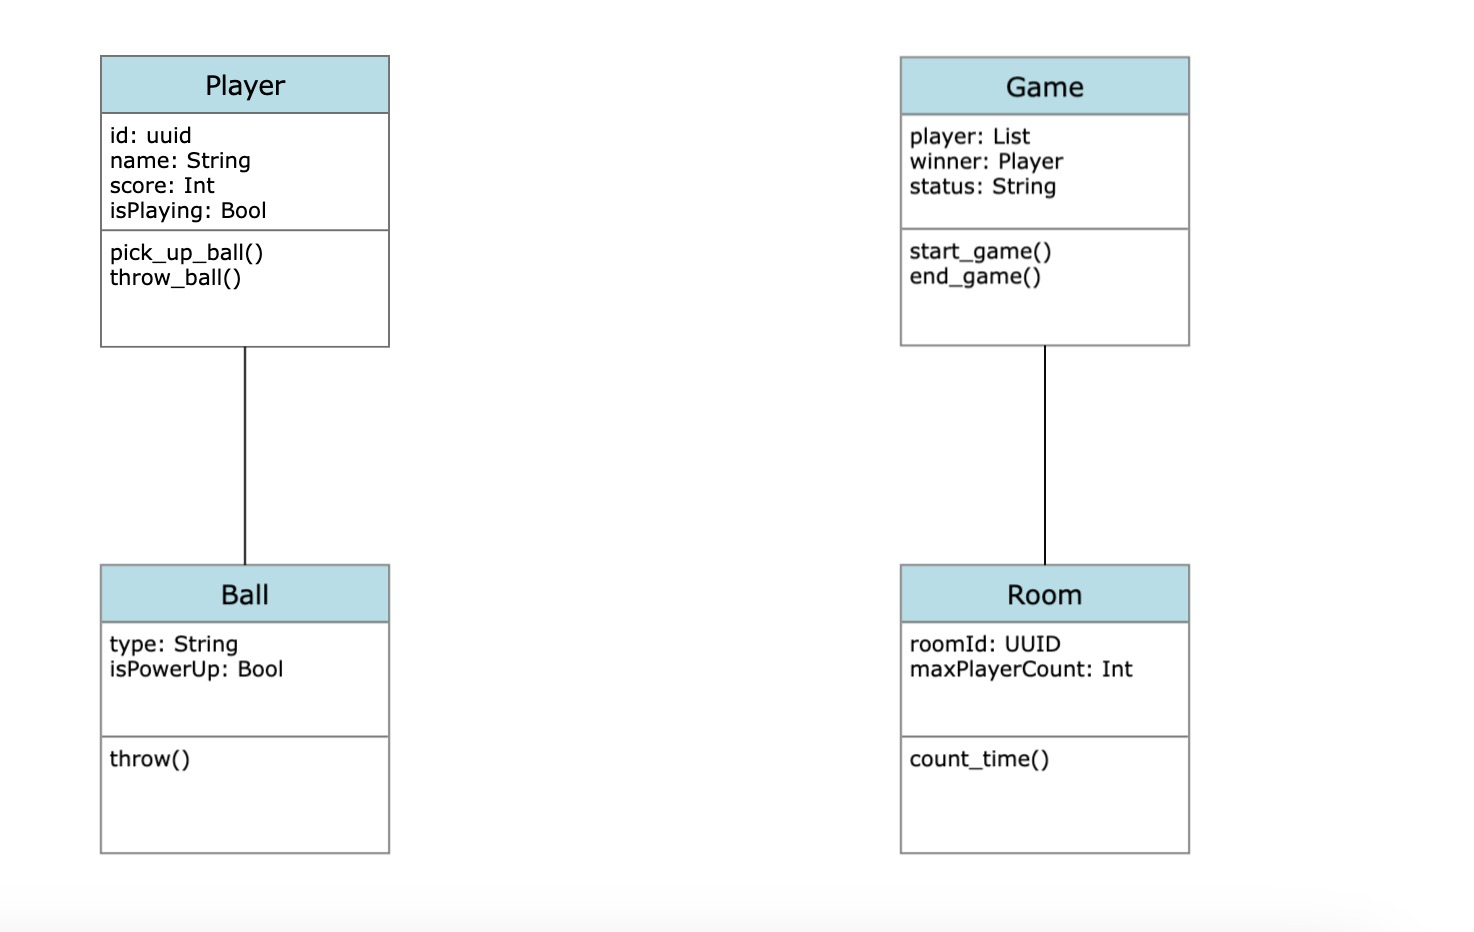
\includegraphics[scale=0.9]{images14.png}

\end{figure}
\vspace{15 cm}


% start of References
\centering
\Large\textbf{REFERENCES}
\justifying
\setlength{\parindent}{4em}
\setlength{\parskip}{0.5em}
\renewcommand{\baselinestretch}{1.5}
\normalsize

\begin{enumerate}


\item Vincenzo Moscato, Antonio Picariello and Giancarlo Sperli. An Emotional Recommender 
System for Music. October 01,2020 at 17:32:18 UTC from IEEE Xplore.

\item Ahlam Alrihaili, Alaa Alsaedi, Kholood Albalawi, Liyakathunisa Syed. Music  
Recommender System for users based on Emotion Detection through Facial Features. une 
22,2020 at 07:44:06 UTC from IEEE Xplore.

\item Metilda Florence, M Uma. Emotional Detection and Music Recommendation System based 
on User Facial Expression. IOP Conf. Series: Materials Science and Engineering 912 
(2020) 062007.

\item Sushmita G. Kambale, Asso. Prof. A.H. Kulkarni. Facial Expression based Music Player. 
Conference on Advances in Computing, Communications and Informatics (ICACCI), 
Sept. 21-24, 2016.

\item B. Naren Sai, D. Sai. Vamshi, Piyush Pogakwar, V. Seetharama Rao, Y. Srinivasulu. 
Music Recommendation System Using Facial Expression Recognition Using Machine 
Learning. ISSN: 2321-9653; IC Value: 45.98; SJ Impact Factor: 7.538 Volume 10 Issue 
VI June 2022.
\item Ziyang Yu1, Mengda Zhao1, Yilin Wu1, Peizhuo Liu1, Hexu Chen, Research On 
Automatic Music Recommendation Algorithm Based On "Facial Micro-Expression 
Recognition”, Proceedings Of The 39th Chinese Control Conference July 27-29, 2020. 
\item Dr. Sunil Bhutada, Ch. Sadhvika, Gutta.Abigna, P. Srinivas Reddy, "Emotion Based 
Music Recommendation System", Jeter April 2020. 
\item Mikhail Rumiantcev, Oleksiy Kiriyenko, "Emotion Based Music Recommendation 
System", Proceeding of the 26th Conference of Fruct Association.

\item Krupa K S, Kartikey Rai, Ambara G, Sahil Choudhury, "Emotion Aware Smart Music 
Recommender System Using Two Level CNN", Third International Conference On Smart 
Systems And Inventive Technology (Icssit 2020).



\end{enumerate}
%\subsubsection{WEB RESOURCES}
%\begin{enumerate}
%\item  \href{URL}{www.wikipedia.org}
%\item  \href{URL}{www.sciencedirect.com}
%\item  \href{URL}{www.slideshare.net}
%\end{enumerate}
\clearpage
%end of references


% seminar report documentation


\end{document}
